\documentclass{report}
\usepackage{graphicx}
\usepackage{amssymb}
\usepackage{amsmath}
\usepackage{float}
\usepackage{xparse}
\newcommand{\subsubsubsection}[1]{\paragraph{#1}\mbox{}\\}
\NewDocumentCommand{\D}{m g}{%
    \IfNoValueTF{#2}{%
        \frac{d}{d#1}
    }{%
        \frac{d^{#2}}{d^{#2}#1}
    }
}
% \newcommand
\title{Calcolo differenziale}

\begin{document}
\maketitle
\section{Equazioni e disequazioni}
    \subsection{La retta}
        \begin{center}
            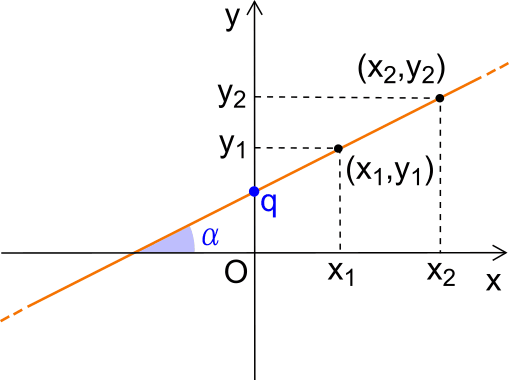
\includegraphics[width=\textwidth]{retta.png}
        \end{center}
        La retta è \textbf{lineare} in x e y. \\
        Se $ m > 0 $ è \textbf{crescente}, se $ m < 0 $ è \textbf{decrescente}.
        \textbf{Forma esplicita} $ y = mx + q $. \\
        Questa forma descrive tutte le rette tranne quella \textbf{verticale}: $ y = c $ \\
        \textbf{Forma implicita} $ ax + by + c = 0 $
        $$ m = tg\Theta = \frac{\Delta y}{\Delta x} $$
        $$ y = m(x - x_0) + y_0 \Longleftrightarrow q = y_0 - mx_0 $$
        $$ ax \geq -b \Longrightarrow $$
        \begin{itemize}
            \item se $a > 0: x \geq \frac{-b}{a} $
            \item se $a < 0: x \leq \frac{-b}{a} $
        \end{itemize}
    \subsection{Polinomi di secondo grado: le parabole}
        \begin{center}
            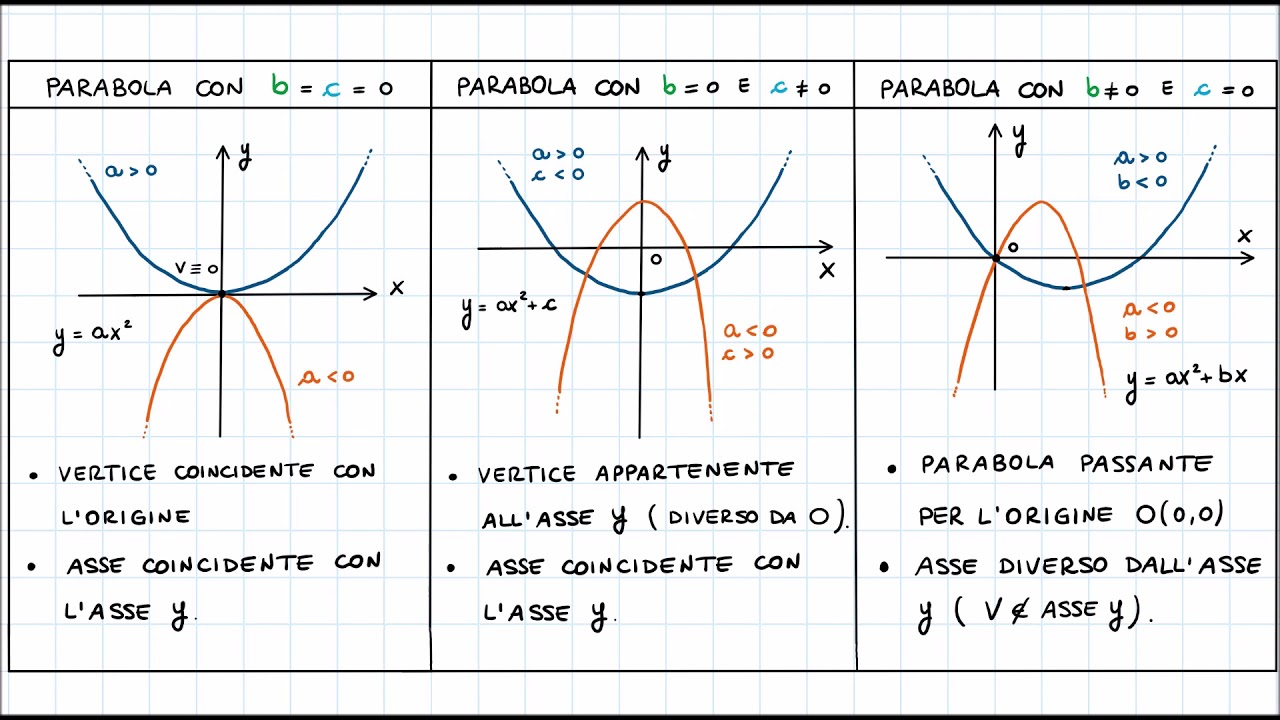
\includegraphics[width=\textwidth]{parabola.jpg}
        \end{center}
        $$ P_2(x) = ax^2 + bx + c, a \neq 0 $$
        $$ x^2 = c \Longrightarrow $$
        \begin{itemize}
            \item se $c > 0: x \pm \sqrt[2]{c} $
            \item se $c = 0: x = 0 $
            \item se $c < 0: \nexists x \in I\!R $
        \end{itemize}
        \subsubsection{Dimostrazione della correttezza della formula risolutiva per le equazioni di secondo grado}
            $$ ax^2 + bx + c = 0, a \neq 0 $$
            $$ a \cdot \left[ x^2 + \frac{bx}{a} + \frac{c}{a} \right] = 0 $$
            $$ x^2 + \frac{bx}{a} + \frac{b^2}{4a^2} - \frac{b^2}{4a^2} + \frac{c}{a} = 0 $$
            $$ \left[ x + \frac{b}{2a} \right]^2 - \frac{b^2}{4a^2} + \frac{c}{a} = 0 $$
            $$ \left[ x + \frac{b}{2a} \right]^2 = \frac{b^2 - 4ac}{4a^2} $$
            $$ x + \frac{b}{2a} = \pm \sqrt[2]{\frac{b^2 - 4ac}{4a^2}} $$
            $$ x = -\frac{b}{2a} \pm \sqrt[2]{\frac{b^2 - 4ac}{4a^2}} $$
            $$ x = \frac{-b \pm \sqrt[2]{b^2 - 4ac}}{2a} $$
            In questa situazione abbiamo 3 opzioni:
            \begin{itemize}
                \item $b^2 - 4ac > 0 \Longleftrightarrow $ 2 soluzioni
                \item $b^2 -4ac = 0 \Longleftrightarrow $ 1 soluzione
                \item $b^2 - 4ac < 0 \Longleftrightarrow $ 0 soluzioni
            \end{itemize}
    \subsection{Modulo}
        $ |x| = \sqrt[2]{x^2} = $
        \begin{itemize}
            \item se $x > 0: x $
            \item se $x < 0: -x $
        \end{itemize}
        Geometricamente, il modulo è \textbf{la distanza} di x dal punto \textbf{0} sull'asse dei numeri $I\!R$. \\
        $$ |x| \leq a \Longleftrightarrow \left[ -a, a \right] $$
        $$ |x| \geq a \Longleftrightarrow \left( -\infty, -a \right] \cup \left[ a, +\infty \right) $$
        $$ -|x| \leq x \leq |x| $$ 
        \textbf{Disuguaglianza triangolare}: $|x + y| \leq |x| + |y|$
        $$ |x \cdot y| = |x| \cdot |y| $$
\section{Insiemi numerici}
    E' detta \textbf{insieme} una \textbf{collezione} di elementi per i quali è 
    sempre possibile rispondere alla domanda $x \in A$.
    \subsection{Applicazioni}
    Tramite un'applicazione, associo gli elementi dell'insieme A
    agli elementi dell'insieme B, detto \textbf{immagine} di A. \\
    Un'applicazione è:
    \begin{itemize}
        \item \textbf{Iniettiva}: $
            \forall x_1, x_2 \in A \textrm{ t.c. } x_1 \neq x_2:
            x_1 \rightarrow b_1 \neq x_2 \rightarrow b_2
        $
        \item \textbf{Suriettiva}: $\forall b \in B: 
            \exists a \in A \textrm{ t.c. } a \rightarrow b
        $
        \item \textbf{Biunivoca}: Suriettiva $\wedge$ Iniettiva
    \end{itemize}
    Se esiste un'applicazione suriettiva ed iniettiva fra $A$ e $B$ questi sono
    detti in \textbf{biezione}.
    \subsection{Definizione di $\mathbf{N}$ tramite gli insiemi}
    A questo punto possiamo definire i numeri naturali positivi partendo dagli insiemi.
    \begin{itemize}
        \item \textbf{0}: classe degli insiemi in biezione con $A = \emptyset$
        \item \textbf{1}: classe degli insiemi in biezione con $A = \{\emptyset\}$
        \item \textbf{2}: Classe degli insiemi in biezione con $A = \{\emptyset, \{\emptyset\}\}$
        \item \textbf{...}: ...
    \end{itemize}
    Possiamo accorgerci quindi come l'insieme $\mathbf{N}$ definisce la \textbf{cardinalità}
    degli insiemi. \\
    Da qui possiamo continuare:
    \begin{itemize}
        \item \textbf{$\mathbf{N} +$}: poichè $\mathbf{N}$ definisce la cardinalità degli insiemi,
            la somma di due numeri $\in \mathbf{N}$ è uguale alla cardinalità di 
            $(A \cup B) \forall A, B \textrm{ t.c. } A \cap B = \emptyset$.
        \item \textbf{-1}: quel numero t.c. $-1 + 1 = 0$. Da qui definiamo $\mathbf{Z}$.
        \item \textbf{$\frac{n}{m}$}: 
            $a_1, a_2, ..., a_n \in \mathbf{Z}, 0 \leq a_2, ..., a_n \leq 9:
            a_1 + \sum_{i=1}^{n}\frac{a^i}{10^i}$
        \item \textbf{$\mathbf{Q}$}: 
            ${\frac{n}{m},\frac{n_1}{m_1} \in \mathbf{Z}, m, m_1 \neq 0: 
            (n, m) = (n_1, m_1) \Longleftrightarrow (n \cdot m_1) = (n_1 \cdot m)}$. \\
            La struttura \textbf{periodica} è valida se si conviene che 
            $a,\overline{9} = a + 1$.
        \item \textbf{$\mathbf{Q} +$}: 
            $\frac{n}{m} + \frac{n_1}{m_1} = \frac{n \cdot m_1 + m \cdot n_1}{m \cdot m_1}$
        \item \textbf{$\mathbf{Q} \cdot$}:
            $\frac{n}{m} \cdot \frac{n_1}{m_1} = \frac{n \cdot n_1}{m \cdot m_1}$
        \item \textbf{$\mathbf{Q}$ inverso}: 
            $\frac{n}{m} \cdot \frac{n}{m}^{-1} = 1 \Longrightarrow 
            \frac{n}{m}^{-1} = \frac{m}{n}, n \neq 0$
        \item \textbf{$\mathbf{R}$}: {Tutti i numeri scritti in forma decimale
            anche con \textbf{infinite} cifre \textbf{non periodiche} dopo la virgola}
    \end{itemize}
    Possiamo infine definire le n-tuple di numeri $\left(a, b, ...\right)$ come
    \textbf{prodotto cartesiano} degli insiemi $A \cdot B \cdot ... = \{(a, b, ...) 
    \forall a \in A \wedge \forall b \in B \wedge ...\}$
    $$\mathbf{N} \subset \mathbf{Z} \subset \mathbf{Q} \subset \mathbf{R}$$
\section{Funzioni}
    \subsection{Definizione}
        Dati due insiemi $A$ e $B$, una funzione con \textbf{dominio} $A$ e 
        \textbf{codominio} B è una qualunque legge che \textbf{ad ogni} elemento
        di $A$ associa \textbf{uno ed uno solo} elemento di $B$.\\
        Può anche essere ad \textbf{n variabili} ed avere quindi n insiemi di partenza
        $$f: A \longrightarrow B \textrm{ t.c. } \forall x \in A \longrightarrow f(x) \in B$$
        Le funzioni \textbf{reali} a variabile \textbf{reale} sono le funzioni
        $$f: A \subset \mathbf{R} \longrightarrow \mathbf{R}$$
    \subsection{Immagine}
        $$ \{f(x) \forall x \in A\} \subset B $$
    \subsection{Grafico di una funzione}
        \subsubsection{Definizione}
            L'insieme dei punti $\mathbf{R}^2$ definiti da 
            $$ g_{\mathbf{R}} = \{(x,f(x)) \forall x \in A\}$$
        \subsubsection{Rappresentazione sul piano}
            Poichè $\mathbf{R}^2$ è rappresentabile sul piano cartesiano anche 
            $g_{\mathbf{R}}$ lo è
        \subsubsection{Proprietà fondamentale della funzione espressa col grafico}
        $$\forall x_0 \in A \, \exists!y_0 \textrm{ t.c. } {x = x_0} \cap {g_{\mathbf{R}}}
            = {(x_0, f(x_0))}$$
    \subsection{Proprietà delle funzioni}
        Una funzione è detta
        \begin{itemize}
            \item \textbf{pari}: $\forall x \in A: f(x) = f(-x)$
            \item \textbf{dispari}: $\forall x \in A: -f(x) = f(-x)$
            \item \textbf{limitata superiormente}: $\exists M \in \mathbf{R} 
                \textrm{ t.c. } M \geq f(x) \forall x \in A$
            \item \textbf{limitata inferiormente}: $\exists m \in \mathbf{R} 
                \textrm{ t.c. } m \leq f(x) \forall x \in A$
            \item \textbf{limitata}: $f(x)$ è limitata superiormente e inferiormente
            \item \textbf{monotona crescente in A}: $\forall x_1, x_2 \in A \textrm{ t.c. } 
                x_1 \leq x_2: f(x_1) \leq f(x_2)$
            \item \textbf{monotona decrescente in A}: $\forall x_1, x_2 \in A \textrm{ t.c. } 
                x_1 \leq x_2: f(x_1) \geq f(x_2)$
            \item \textbf{periodica di periodo T}: $\forall x \in A, x + kT \in A, 
                k \in \mathbf{Z}: f(x + kT) = f(x)$
            \item \textbf{successione}: il dominio è $\mathbf{N}$, $f(n) = a_n$
        \end{itemize}
    \subsection{Funzioni composte}
    \begin{itemize}
        \item $g(f(x)) = g \circ f(x)$
        \item \textbf{funzione neutra o identità}: $f(x) = x = I(x)$
        \item \textbf{funzione inversa}: $f \circ f^{-1}(x) = f^{-1} \circ f(x) = I(x)$
        \item $f^{-1}: \textrm{Img}_f \rightarrow \textrm{Def}_f$
    \end{itemize}
        \subsection{Condizioni di esistenza della funzione inversa}
            \begin{itemize}
                \item Img$_f \subset Def_g$ 
                \item f \textbf{iniettiva}: se, per assurdo, non lo fosse vorrebbe dire 
                    che $\exists x_1,x_2 \textrm{ t.c. } x_1 \neq x_2, \, \, y_1 = f(x_1) = f(x_2)$ e quindi
                    $f^{-1}(y)$ potrebbe essere sia $x_1$ che $x_2$, e quindi $f^{-1}$
                    non sarebbe una funzione
            \end{itemize}
    \subsection{Operazioni sui grafici}
        \begin{itemize}
            \item $f(x+k)$: spostamento a sx
            \item $f(x-k)$: spostamento a dx
            \item $f(x) + k$: spostamento in alto
            \item $f(x) - k$: spostamento in basso
            \item $-f(x)$: ribaltamento su asse y
            \item $(f(-x))$: ribaltamento su asse x
            \item $|f(x)|$: ribaltamento su asse x degli $y < 0$
            \item $f(|x|)$: Ribaltamento su asse y della funzione quando $x < 0$
        \end{itemize}
    \subsection{Funzioni continue}
        \subsubsection{Criterio di continuità}
            Riferirsi al capitolo presente nei limiti di funzioni
        \subsubsection{Teorema di esistenza degli zeri}
            $$f:\left[a, b\right] \longrightarrow \mathbf{R}, \, f \textrm{ continua }$$
            $$f\left(a\right) \cdot f\left(b\right) < 0 \Longrightarrow \exists x_0 \in 
                \left(a, b\right) \textrm{ t.c. } f\left(x_0\right) = 0$$
            \subsubsubsection{Dimostrazione}
                Ipotizziamo $f\left(a\right) < 0 \wedge f\left(b\right) > 0$. \\
                Usiamo \textbf{l'algoritmo di biezione} per arrivare a $x_0$ t.c. $f\left(x_0\right) = 0$. \\
                \begin{enumerate}
                    \item $c = \frac{a + b}{2}$
                    \item 3 casi:
                        \begin{enumerate}
                            \item $f\left(c\right) > 0 \Longrightarrow x_0 \in \left[a, c\right]$
                            \item $f\left(c\right) = 0 \Longrightarrow x_0 = c$. Abbiamo dimostrato che esiste $x_0$
                            \item $f\left(c\right) > 0 \Longrightarrow x_0 \in \left[c, b\right]$
                        \end{enumerate}
                    \item Applico ricorsivamente l'algoritmo sul nuovo intervallo ottenuto al passo 2
                \end{enumerate}
                Dobbiamo quindi dimostrare che, eventualmente, questo procedimento arrivi al caso 2 del punto 2. \\
                Prendiamo ora la successione di tutti gli estremi sinistri costruiti fino al punto n degli intervalli (tutte le $a$) e chiamiamola
                $\{a_n\}_n$ e la successione di tutti gli estremi destri (tutte le $b$) e chiamiamola $\{b_n\}_n$. \\
                Per come lo costruiamo, sappiamo che:
                \begin{itemize}
                    \item $a_{n} > a_{n-1}, \, a_n < b \, \forall n$
                    \item $b_{n} < b_{n-1}, \, b_n > a \, \forall n$
                    \item In quanto limitate e monotone $\in \left[a, b\right]$, $\lim_{n \to \infty} a_n = sup_a, \, \lim_{n \to \infty} b_n = inf_b$
                    \item $b_{n} - a_{n} = \frac{b - a}{2^n}$ (L'intervallo dimezza ad ogni passo)
                    \item $\forall n \, f\left(a_n\right) \leq 0, f\left(b_n\right) \geq 0$ per come scegliamo $a_n$ e $b_n$
                \end{itemize}
                Il quarto punto ci permette di concludere che:
                $$\lim_{n \to \infty} b_n - a_n = \frac{b - a}{2^n} = 0 \Longrightarrow \lim_{n \to \infty} b_n = \lim_{n \to \infty} a_n$$
                $$\Longrightarrow sup_a = inf_b$$
                Quindi, posto $c = sup_a = inf_b$, e per il teorema della permanenza del segno 
                $f\left(a_n\right) \cdot \left(b_n\right) \leq 0 \Longrightarrow f\left(c\right)^2 \leq 0 $
                volendo dimostrare che $f\left(c\right) = 0$ per l'algoritmo di biezione, 
                partiamo dalle cose che sappiamo:
                $$f\left(a_n\right) \cdot f\left(b_n\right) \leq 0$$
                $$\lim_{n \to \infty} f\left(a_n\right) \cdot f\left(b_n\right) = f\left(c\right)^2 \geq 0 \textrm { in quanto quadrato }$$
                $$\Longrightarrow f\left(c\right)^2 \geq 0 \wedge f\left(c\right)^2 \leq 0 \Longrightarrow f\left(c\right)^2 = 0$$
                $$\Longrightarrow f\left(c\right) = 0 \textrm{ c.v.d. }$$
            \subsubsubsection{Corollario}
                $$f: \left[a, b\right] \longrightarrow \mathbf{R}, \, f \textrm{ continua e strettamente monotona}$$
                $$f\left(a\right) \cdot f\left(b\right) < 0 \Longrightarrow 
                    \exists! x_0 \in \left[a, b\right] \textrm{ t.c. } f\left(x_0\right) = 0$$
        \subsubsection{Teorema di Weiestrass}
            $$f: \left[a, b\right], a \neq -\infty, b \neq +\infty, \longrightarrow \mathbf{R}, \, f \textrm{ continua }$$
            $$\exists m, M \textrm{ di } f \textrm{ in } \left[a, b\right]$$
            \subsubsubsection{Dimostrazione}
                La dimostrazione che segue è per il massimo, ma il ragionamento per il minimo è analogo
                La premessa fondamentale è che presi due insiemi $I_1, I_2, \sup\left(I_1 \cup I_2\right) = \max\left(\sup I_1, \sup I_2\right)$ \\
                Consideriamo ora $\left[a, b\right] = I_1 \cup I_2 \implies f\left(\left[a, b\right]\right) = f\left(I_1\right) \cup f\left(I_2\right)$ \\
                Quindi $\sup f\left(\left[a, b\right]\right) = \max\left(\sup f\left(I_1\right) \cup \sup f\left(I_2\right)\right)$ \\
                Ne consegue che $sup f\left(\left[a, b\right]\right) = \sup f\left(I_1\right) \lor \sup f\left(I_2\right)$ \\
                Costruiamo ora $\left[a_1, b_1\right]$ come la metà di $\left[a, b\right]$ tale che $sup f\left(\left[a, b\right]\right) = \sup f\left(I_1\right)$. \\
                Possiamo ripetere questo processo infinite volte su $\left[a_{n+1}, b_{n+1}\right] \subset \left[a_n, b_n\right]$ \\
                Possiamo osservare come per costruzione:
                    \begin{itemize}
                        \item $a_n$ è una successione monotona crescente e $b_n$ monotona decrescente. 
                        \item $b_n - a_n = \frac{b - a}{2^n} \rightarrow 0$ per $n \rightarrow \infty$
                        \item $M = \sup f\left(\left[a_n, b_n\right]\right)$
                    \end{itemize}
                In modo analogo al teorema degli zeri dimostriamo che $a_n \rightarrow x_0 \leftarrow b_n$ \\
                Se $M < \infty$ allora 
                $$\forall n \, \exists t_n \in \left[a_n, b_n\right] \textrm{ t.c. } M - \frac{1}{n} < f\left(t_n\right) \leq M$$
                In quanto $M - \frac{1}{n}$ è minore del minimo dei maggioranti questo processo può essere ripetuto (facile notare 
                come possa essere ripetuto infinite volte). \\
                Inoltre, per il teorema del confronto, $t_n \rightarrow x_0$. Ne consegue che 
                $$\lim_{n \to \infty} M - \frac{1}{n} < f\left(t_n\right) < M = M - 0 < f\left(x_0\right) \leq M \implies f\left(x_0\right) = M$$ \\
                Se invece $M = \infty$, ne segue che $\forall n \in t_n \in \left[a_n, b_n\right] \textrm{ t.c. } f\left(t_n\right) > M$ \\
                Ma se $t_n \rightarrow x_0$ allora $\lim_{n \to \infty} f\left(t_n\right) = f\left(x_0\right) = \infty$, impossibile in 
                quanto $f\left(x_0\right) \in \mathbf{R} - \{-\infty, +\infty\}$
        \subsubsection{Teorema del valore intermedio avanzato}
            $$f: \left[a, b\right] \longrightarrow \mathbf{R}, f \textrm{ continua }$$
            $$\Longrightarrow f\left(\left[a,b\right]\right) = \left[m, M\right]$$
            La dimostrazione deriva dall'uso del teorema di Weiestrass e dal teorema degli 
            zeri per la funzione $g\left(x\right) = f\left(x\right) - y \, \forall y \in \left[m, M\right]$
        \subsubsection{Algebra delle funzioni continue}
            $$f, g: \left[a, b\right], x_0 \in \left[a, b\right], \, f, g \textrm{ continue } \Longrightarrow$$
            \begin{itemize}
                \item $f\left(x_0\right) \pm g\left(x_0\right)$ continua
                \item $f\left(x_0\right) \cdot g\left(x_0\right)$ continua
                \item $f\left(x_0\right) / g\left(x_0\right)$ continua purchè $g\left(x_0\right) \neq 0$
            \end{itemize}
        \subsubsection{Teorema del cambio di variabile}
        $$f, g, \, f \circ g \textrm{ ben definita per }x \rightarrow x_0$$
        $$\lim_{x \to x_0} g\left(x\right) = t_0, \exists \lim_{t \to t_0} f\left(t\right) = l$$
        $$\textrm{Inoltre, nel caso } f \textrm{ sia non continua in } t_0 \textrm{ o }t_0 = \pm \infty, 
            g\left(x_0\right) \neq t_0$$
        $$\Longrightarrow \lim_{x \to x_0} f\left(g\left(x\right)\right) = \lim_{t \to t_0} f\left(t\right)$$
        \subsubsection{Continuità della funzione composta}
            $$g: \left[a, b\right], f: \left[c, d\right], x_0 \in \left[a, b\right], g\left(x_0\right) \in \left[c, d\right]$$
            $$f, g \textrm{ continue } \Longrightarrow f\left(g\left(x_0\right)\right): 
                \left[a, b\right] \textrm{ e continua in }x_0$$
        \subsubsection{Teorema di esistenza della radice i-esima}
            $$\forall y \in \mathbf{R}, n \in \mathbf{N}, \textrm{ t.c. } y > 0, n \geq 1$$
            $$\Longrightarrow \exists! x \in \mathbf{R}, x > 0 \textrm { t.c. } x^n = y$$
            \subsubsubsection{Dimostrazione}
            $$g\left(x\right) = x, \, \textrm{ continua }, f\left(x\right) = x^n = \Pi_{1}^{n}g\left(x\right)
                \Longrightarrow, f\left(x\right) \textrm{ continua }$$
            $$ \left\{\begin{matrix} 
                    1^n \leq y \leq y^n & y \geq 1, \, x_1 = 1, x_2 = y \\
                    y^n \leq y \leq 1^n & y < 1, \, x_1 = y, x_2 = 1 \\
                \end{matrix} \right\}
                f\left(x\right) \textrm{ strettamente monotona } \in \left[x_1, x_2\right] \Longrightarrow x_1^n = m, x_2^n = M
            $$
            $$\Longrightarrow \textrm{ per il teorema dei valori intermedi } \exists !x_0 \in \left[x_1, x_2\right]
                \textrm{ t.c. } f\left(x_0\right) = x_0^n = y$$
    \subsection{Funzioni monotone}
        \subsubsection{Teorema di monotonia}
            $$f:\left(a, b\right), f \textrm{ monotona }$$
            $$\Longrightarrow \forall c \in \left(a, b\right) \exists \textrm{ finiti limite 
            destro e sinistro per } x \rightarrow c \textrm{ e limite sinistro/destro per } x \rightarrow a/b$$
            \subsubsubsection{Dimostrazione}
                $S = sup\{f\left(x\right) \forall x \in \left(a, c\right)\}$, $S$ finito in quanto $S = f\left(c\right)$ per monotonia \\
                Dobbiamo provare che
                $$\lim_{x \to c^-} f\left(x\right) = S$$
                ovvero che, presa la successione $x_n \in \left(a, c\right)\textrm{ t.c. } x_n \rightarrow c$,
                $$\forall\epsilon > 0, S-\epsilon < f\left(x_n\right) < S+\epsilon$$
                $$S > f\left(x\right) \forall x \in \left(a, c\right) \Longrightarrow S+\epsilon > f\left(x_n\right) \forall n$$
                $$S > S-\epsilon \Longrightarrow \exists x_0 \in \left(a, c\right) \textrm{ t.c. } f\left(x_0\right) \geq S-\epsilon$$
                $$\Longrightarrow f\left(x\right) \geq S-\epsilon \, \forall x \in \left(x_0, c\right) \textrm{ perchè monotona } \Longrightarrow f\left(x_n\right) \geq S-\epsilon$$
                $$\Longrightarrow x_n \in \left(x_0, c\right) \textrm{ definitivamente } \Longrightarrow f\left(x_n\right) \geq S - \epsilon \textrm{ definitivamente }$$
                $$\Longrightarrow \lim_{x \to c^-} f\left(x\right) = S$$
                Analogamente possiamo fare con $\lim_{x \to c^+} f\left(x\right)$. \\
                Per i limiti agli estremi possiamo usare lo stesso procedimento, ricordando però che $S, s$ non 
                sono necessariamente finiti in quanto $f\left(b/a\right)$ non sono maggioranti/minoranti in quanto 
                la funzione non è definita in $a, b$. La dimostrazione cambia se $S = \infty$:
                $$S = \infty \implies \forall K > 0 \exists x_0 \in \left(a, b\right) \textrm{ t.c. } f\left(x_0\right) > K$$
                $$\Longrightarrow f\left(x\right) > K \, \forall x \in \left(x_0, b\right)$$
                Presa una successione $x_n \rightarrow b, x_n \in \left(x_0, b\right)$
                $$\Longrightarrow f\left(x_n\right) > K \textrm{ definitivamente }$$
                $$\Longrightarrow \lim_{x \to b^-} f\left(x\right) = \infty$$
                Nel caso la funzione sia decrescente anzichè crescente cambiare in modo appropriato.
            \subsubsubsection{Corollario}
                $$f:\left(a, b\right), f \textrm{ monotona }$$
                Se esistono dei punti di discontinuità in $\left(a, b\right)$ questi
                sono necessariamente \textbf{punti di salto}
    \subsection{Teorema di invertibilità della funzione continua}
        $$f: \left(a, b\right), f \textrm{ continua }$$
        $$\Longrightarrow \exists f^{-1}: \left(a, b\right), f^{-1}\textrm{ strettamente monotona e continua } 
            \Longleftrightarrow f \textrm{ strettamente monotona }$$
        \subsubsection{Dimostrazione}
            \subsubsubsection{Dimostrazione prima parte}
                Dimostriamola per contrapposizione con $f$ non strettamente monotona. Vuol dire che
                $$\exists x_0 < x_1 < x_2 \in \left(a, b\right) \textrm{ t.c. } f\left(x_0\right) \leq f\left(x_1\right) \geq f\left(x_2\right)$$
                Per il teorema dei valori intermedi
                $$\exists c \in \left(x_0, x_1\right) \textrm{ t.c. } f\left(c\right) = f\left(x_2\right) \wedge c \neq x_2$$
                La funzione non è quindi invertibile
            \subsubsubsection{Dimostrazione seconda parte}
                Prendiamo $f^{-1}$ che sappiamo essere monotona ed ipotizziamo non sia continua. 
                Per il teorema di monotonia sappiamo che i suoi punti di discontinuità in $f^{-1}$ 
                sono punti di salto, e quindi l'immagine di $f^{-1}$ non sarebbe un intervallo in quanto strettamente monotona.
                Impossibile in quanto l'immagine di $f^{-1} = \left[a, b\right]$
\section{Limiti di successioni}
    \subsection{Disuguaglianza di bernoulli}
        $$n \geq 0,\, x > -1, \Longleftrightarrow \left(1+x\right)^n \geq 1 + nx$$
    \subsection{Limiti convergenti}
        Una successione è detta \textbf{convergente} a $l$, o $\lim_{x \to \infty} = l$ se 
        $$\forall\epsilon > 0,\, \exists N = N\left(\epsilon\right) \textrm{ t.c. } \forall n > N \Longrightarrow
        |a_n - l| \leq \epsilon$$
        Non tutte le successioni convergono.
    \subsection{Limiti divergenti}
        Una successione è detta \textbf{divergente} a $+\infty$, o 
        $\lim_{x \to \infty} = +\infty$, se $$\forall M > 0, \exists N = N\left(M\right)
        \textrm{ t.c. } \forall n > N \Longrightarrow a_n \geq M$$ e divergente a 
        $-\infty$ se $a \leq -M$. \\
        Non tutte le successioni divergono.
        \subsubsection{Convergenza per eccesso e per difetto}
            Una successione è detta tendere ad l per \textbf{eccesso} (l$^+$) nel caso 
            in cui a$_n >$ l, per \textbf{difetto}(l$^-$) in caso contrario.
    \subsection{Monotonia e limiti}
        Preso $A = \{a_n \forall n \in \mathbf{N}\}$, se $a_{n \in \mathbf{N}}$ è una successione \textbf{monotona}:
        \begin{itemize}
            \item \textbf{crescente}: converge a sup$_A$ se limitata, se no diverge a $+\infty$
            \item \textbf{decrescente}: converge ad inf$_A$ se limitata, se no diverge a $-\infty$
        \end{itemize}
    \subsubsection{Numero di nepero}
        La convergenza di $a_n$: $\lim_{n \to \infty} \left(1+\frac{1}{a_n}\right)^n = e$
        \subsubsubsection{Dimostrazione}
            Dimostriamo che è monotona crescente
            $$\begin{array}{c}
                \left(1 + \frac{1}{n}\right)^n = \sum_{k = 0}^n \binom{n}{k}\frac{1}{n^k} \\ \\
                = \sum_{k = 0}^n \frac{n \cdot \left(n-1\right) ... \cdot \left(n-k+1\right)}{k!} \cdot \frac{1}{n^k} \\ \\
                = \sum_{k = 0}^n \frac{1}{k!} \cdot \Pi_{j = 0}^{k-1} 1 - \frac{j}{n} \\ \\
                \implies \\  \\
                \left(1 + \frac{1}{n+1}\right)^{n+1} = \sum_{k = 0}^n\frac{1}{k!} \cdot \Pi_{j=0}^{k-1} 1 - \frac{j}{n+1}
            \end{array}$$
            Possiamo notare subito come ogni termine del prodotto per del caso $n+1$ sia maggiore del corrispettivo termine del caso $n$, di consegunza 
            ogni prodotto del caso $n+1$ è maggiore, il che implica che è maggiore anche la somma. Quindi possiamo affermare che $a_{n+1} > a_n$. \\
            Dimostriamo ora che limitata superiormente: \\
            $$k! \geq 2^{k-1} \implies \frac{1}{k!} \leq \frac{1}{2^{k-1}}$$
            Inoltre, in quanto i fattori della moltiplicazione interna della sommatoria sono $\leq 1$, ne consegue che il prodotto è $\leq 1$, il che implica
            $$\sum_{k=0}^n \frac{1}{k!} \cdot \Pi_{j = 0}^{k-1}  1 - \frac{j}{n} \leq \sum_{k=0}^n \frac{1}{k!} \leq \sum_{k=0}^n \frac{1}{2^{k-1}}$$
            $$\sum_{k=0}^n \frac{1}{2^{k-1}} = 1 + \sum_{k = 0}^{n-1}\frac{1}{2^k} = 1 + 2 \cdot \left(1 - \frac{1}{2^n}\right) < 3$$
            Quindi 
            $$\sum_{k=0}^n \frac{1}{k!} \cdot \Pi_{j = 0}^{k-1}  1 - \frac{j}{n} < 3$$
            Ne consegue che la successione converge
    \subsection{Algebra dei limiti}
        Con $\lim_{n \to n_0} a_n = a$ \\
        $\lim_{n \to n_0} a_n + b_n = a + b$ \\
        $\lim_{n \to n_0} a_n \cdot b_n = a \cdot b$ \\
        $\lim_{n \to n_0} a_n^{b_n} = a^b$ \\
        $\lim_{n \to n_0} f(a_n) = f(a)$ \\
    \subsection{Teorema di permanenza del segno}
        $\lim_{n \to n_0} a_n = a, \, a \geq 0 \Longrightarrow \exists N \in \mathbf{N} \textrm{ t.c. }
            \forall n > N: a_n \geq 0$ \\
        $\lim_{n \to n_0} a_n = a, \, a \leq 0 \Longrightarrow \exists N \in \mathbf{N} \textrm{ t.c. }
            \forall n > N: a_n \leq 0$ \\
        E' quindi implicato: \\
        $\lim_{n \to n_0} a_n = a, \, \lim_{n \to n_0} b_n = b, \, \exists N \textrm{ t.c. } a_n > b_n \forall n \geq N \Longrightarrow a > b$
    \subsection{Teorema dei carabinieri}
        $a_n \leq b_n \leq c_n$
        $a = c \Longrightarrow a = b = c$
        \subsubsection{Dimostrazione}
            $$a_n \rightarrow l \leftarrow c_n \implies l - \epsilon < a_n \leq b_n \leq c_n < l + \epsilon 
                \implies l - \epsilon < b_n < l + \epsilon \implies b_n \rightarrow l$$
        \subsubsection{Corollario}
            $$c_n \rightarrow 0, |b_n| \leq c_n \implies -c_n \leq b_n \leq c_n \implies 0 \leq b_n \leq 0 \implies b_n \rightarrow 0$$
            $$\begin{array}{c}
                b_n \textrm{ limitata }, c_n \rightarrow 0 \implies \forall n |b_n| \leq K, K \geq 0 \\
                \implies |b_n| \cdot |c_n| < K \cdot |c_n| \implies |b_n \cdot c_n| < K \cdot |c_n| \implies |b_n \cdot c_n| < 0 \\
                \implies b_n \cdot c_n \rightarrow 0 \\
            \end{array}$$
    \subsection{Stime asintotiche}
        Prese due successioni che tendono a $\infty$/$0$, considerando 
        $$\lim_{n \to \infty}\frac{a_n}{b_n} = $$
    \begin{itemize}
        \item $0$: $a_n$ è un infinito/infinitesimo di ordine inferiore/superiore a $b_n$
        \item $l, \, \textrm{finito e } \neq 0$: $a_n$ e $b_n$ sono dello stesso ordine. \\
        \item $\pm \infty$: $a_n$ è un infinito/infinitesimo di ordine superiore/inferiore a $b_n$
        \item $\nexists$: $a_n$ e $b_n$ non sono confrontabili.
    \end{itemize}
    \subsubsection{Ordine delle stime asintotiche}
        $$\log_{\alpha}n < n^{\alpha} < \alpha^n < n! < n^n$$ 
    \subsubsection{Successioni asintotiche}
        Nel caso analizzato, quando $l = 1$, diciamo che $a_n$ e $b_n$ sono 
        asintotiche ($a_n \sim b_n$). \\
        \begin{itemize}
            \item $a_n \sim b_n \Longrightarrow$ le due successioni hanno lo stesso comportamento
            \item $a_n \sim b_n \sim c_n \Longrightarrow a_n \sim c_n$
            \item $a_n \sim a^{'}_n, b_n \sim b^{'}_n, c_n \sim c^{'}_n \Longrightarrow 
                \frac{a_nb_n}{c_n} \sim \frac{a^{'}_nb^{'}_n}{c^{'}_n}$
        \end{itemize}
    \subsubsection{Criterio del rapporto}
    $$\lim_{n \to \infty} \frac{a_{n+1}}{a_n} = $$
    \begin{itemize}
        \item $l < 1$: $\lim_{n \to \infty}a_n = 0$
        \item $l > 1$: $\lim_{n \to \infty}a_n = \infty$
        \item $= 1$: non possiamo concludere nulla
    \end{itemize}
\section{Limiti di funzioni}
    \subsection{Definizione tramite limiti di successioni}
        $$x_0 \in I \subset \mathbf{R}, \, l \in \mathbf{R} \cup \{\pm\infty\}$$
        $$f: I\backslash\{x_0\} \longrightarrow \mathbf{R}, \textrm{ se }$$
        $$\forall \textrm{ successione } \{x_n\} \in I\backslash\{x_0\} \textrm { t.c. }
            \lim_{n \to \infty} x_n = x_0, \textrm { si ha che } \lim_{n \to \infty} f\left(x_n\right) = l $$
        $$ \Longrightarrow \lim_{x \to x_0} f\left(x\right) = l $$
    \subsection{Limite da destra e da sinistra}
        $$\lim_{x \to x_0^{\pm}} f\left(x\right) = l$$ studia il comportamento
        della funzione da destra/sinistra.
    \subsection{Criterio d'esistenza del limite}
        Il limite esiste $
            \Longleftrightarrow \lim_{x \to x_0^+} f\left(x\right) = \lim_{x \to x_0^-} f\left(x\right)
        $
    \subsection{Teorema di unicità del limite}
        $$\exists \lim_{x \to x_0} f\left(x\right) = l \Longrightarrow \exists! \lim_{x \to x_0} f\left(x\right) = l$$
    \subsection{Limite per eccesso o per difetto}
        $\exists I\backslash\{x_0\} \textrm{ t.c. } \forall x \in I f\left(x\right) \geq/\leq l \Longrightarrow 
            \lim_{x \to x_0} f\left(x\right) = l$ per eccesso/difetto 
    \subsection{Asintoti}
        Gli asintoti sono rette che approssimano il comportamento della funzione in determinati punti, o verso gli estremi,della stessa.
        I limiti possono tendere da sinistra/destra/bilateralmente
        \subsubsection{Asintoto orizzontale}
            $$\lim_{x \to \pm \infty} f\left(x\right) = l \Longrightarrow \exists \textrm{ asintoto orizzontale } y = l \in \mathbf{R}$$
        \subsubsection{Asintoto verticale}
            $$\lim_{x \to x_0} f\left(x\right) = \pm \infty \Longrightarrow \exists \textrm{ asintoto verticale } x = \pm \infty$$
        \subsubsection{Asintoto obliquo}
            Se $\lim_{x \to \pm \infty} f\left(x\right) = \pm \infty$,   può capitare che presenti limiti obliqui.
            $$\lim_{x \to \pm \infty} \frac{f\left(x\right)}{x} = m, \, \lim_{x \to \pm \infty} |f\left(x\right) - mx| = q$$
    \subsection{Continuità di una funzione tramite limite}
        $$f: I \longrightarrow \mathbf{R}$$
        $$\forall x_0 \in I \lim_{x \to x_0} f\left(x\right) = f\left(x_0\right) \Longrightarrow \textrm{ f è continua in }I$$
    \subsection{Punti di discontinuità}
        \subsubsection{Punto di salto (o prima specie)}
            $lim_{x \to x_0^+} f\left(x\right) \neq lim_{x \to x_0^-} f\left(x\right) \Longrightarrow$ \\
            $\exists \textrm{ punto di salto in } x_0, \, \textrm{ salto in }x_0 = \lim^+ - \lim^-$
        \subsubsection{Punto di discontinuità di seconda specie}
            $$\begin{array}{c}
                \nexists \lim_{x \to x_0^+} f\left(x\right) \vee = \infty \\
                \vee \\
                \nexists \lim_{x \to x_0^-} f\left(x\right) \vee = \infty \\ 
                \Longrightarrow x_0 \textrm{ punto di discontinuità di seconda specie}
            \end{array}$$
        \subsubsection{Discontinuità eliminabile (o di terza specie)}
            $$\begin{array}{c}
                \exists \lim_{x \to x_0} f\left(x\right) = l \wedge l \neq f\left(x_0\right) \vee \nexists f\left(x_0\right) \\
                \Longrightarrow x_0 \textrm{ discontinuità eliminabile }
            \end{array}$$

\newpage
\section{Limiti notevoli}
    \begin{center}
        \hspace*{-1.85in}
        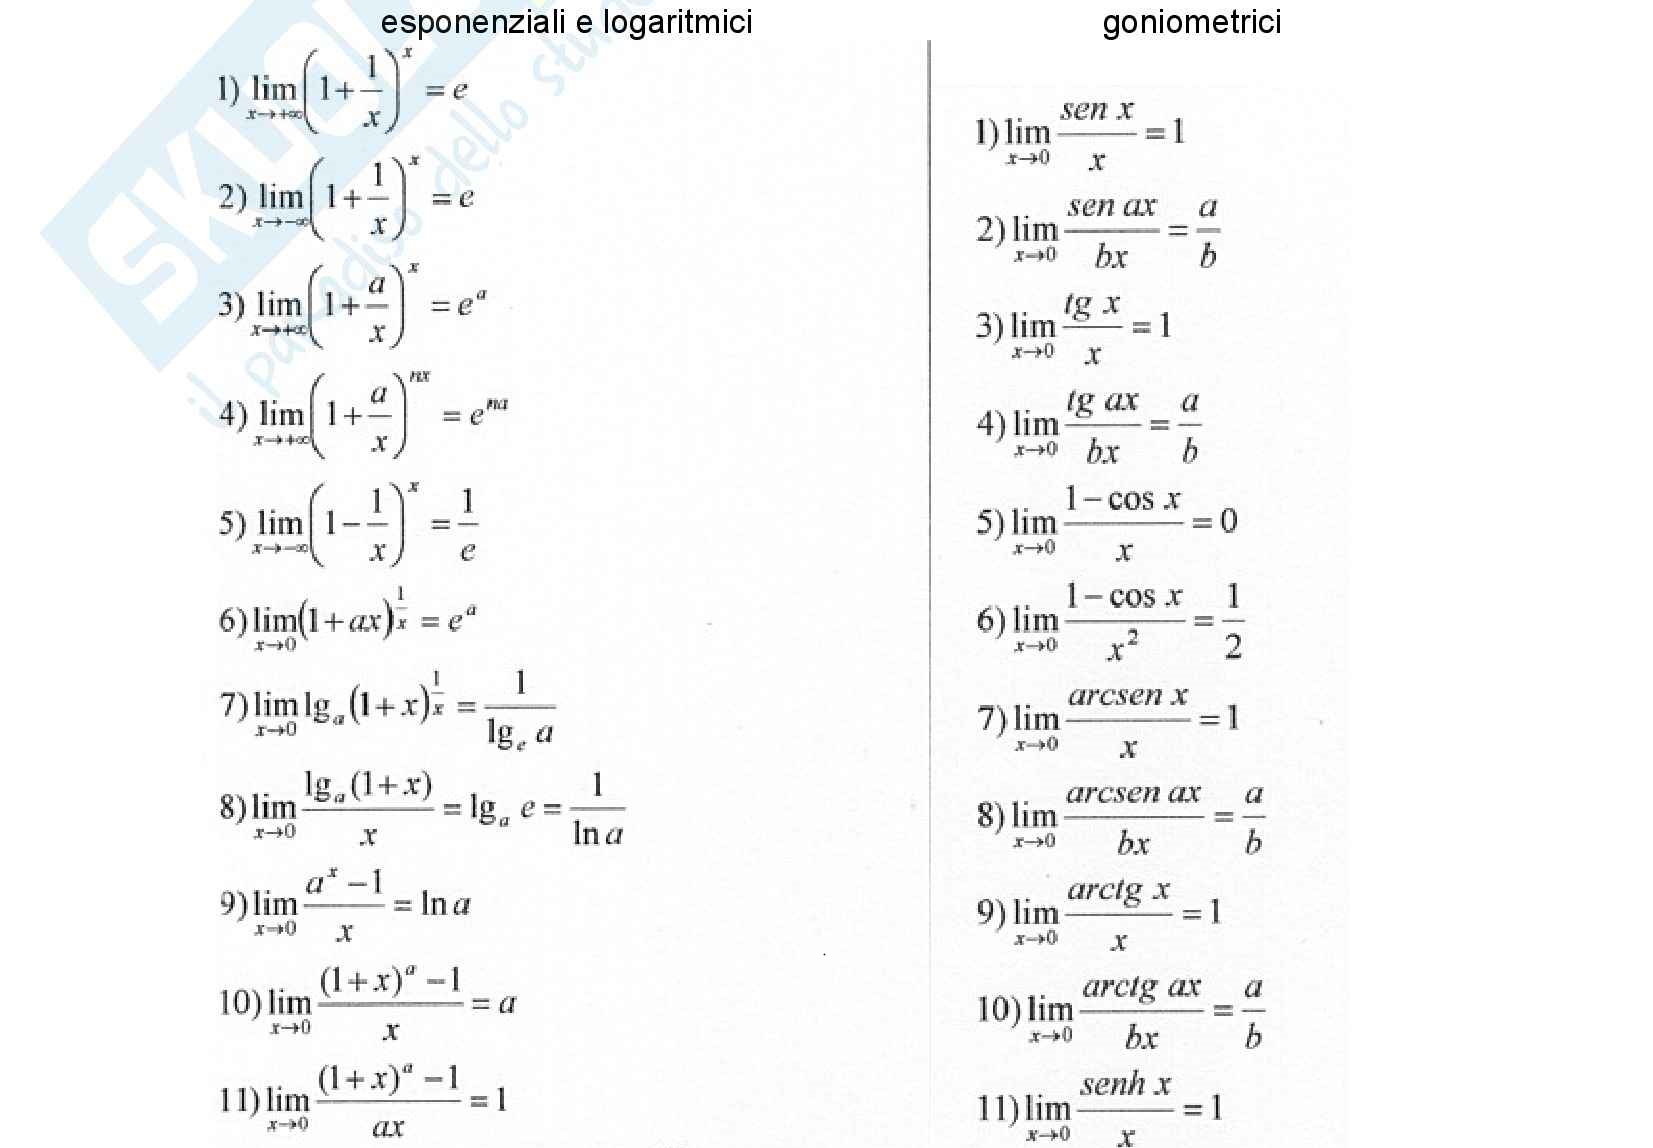
\includegraphics[width=2\textwidth]{limiti-notevoli1.jpg}
        \hspace*{-1.85in}
        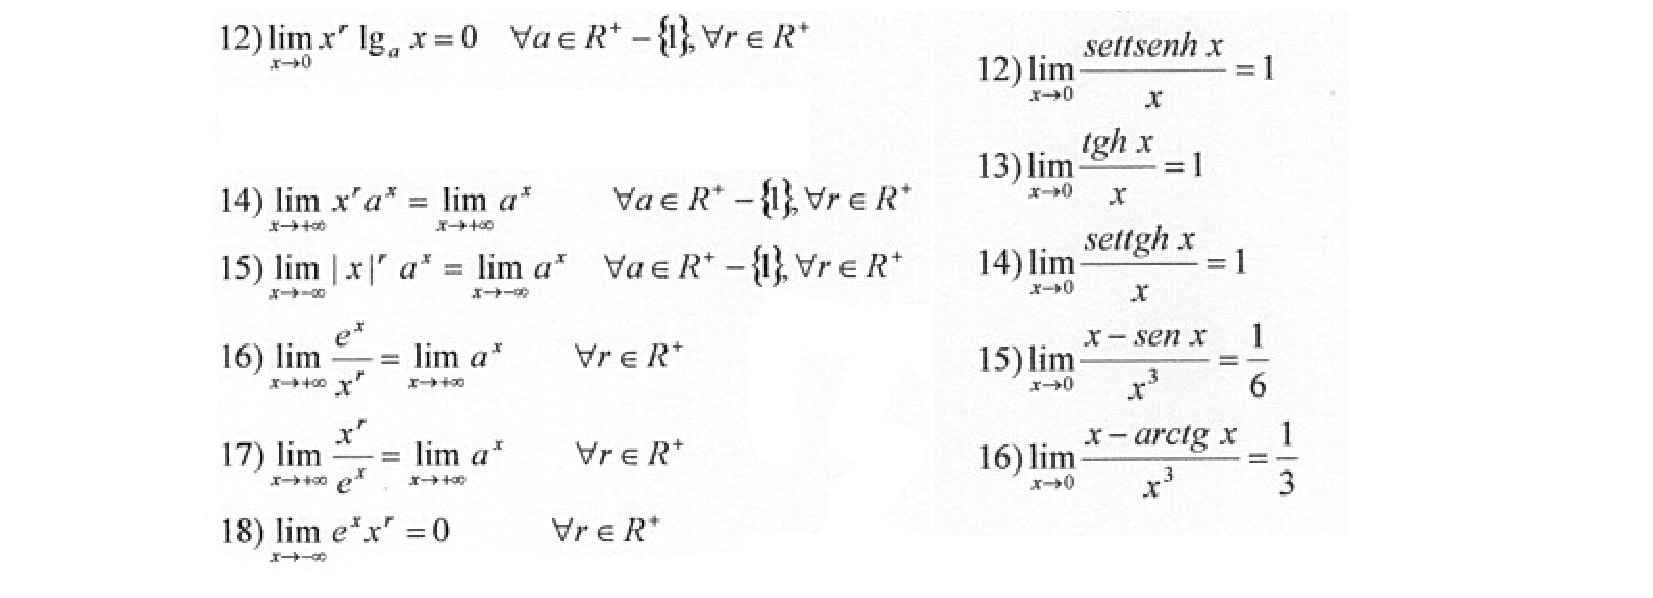
\includegraphics[width=2\textwidth]{limiti-notevoli2.jpg}
    \end{center}
\newpage
\section{Derivate}
    \subsection{Rapporto incrementale}
        R.I.:
        $$\frac{f\left(x+h\right) - f\left(x\right)}{h} = \frac{\Delta y}{\Delta x}$$
    \subsection{Derivata come limite del rapporto incrementale}
        $$f^{'}\left(x\right) = \lim_{h \to 0} \frac{\left(x+h\right) - f\left(x\right)}{h}$$
    \subsection{Punti di non derivabilità}
        Esistono vari tipi di punti di non derivabilità. Di seguito i più interessanti
        \subsubsection{Punto angoloso}
            $$\begin{array}{c}
                \lim_{h \to 0^-} \textrm{R.I.} = l_1 \neq  l_2 = \lim_{h \to 0^+} \textrm{R.I.} \\
                l_1 \vee l_2 \textrm{ finito/i }
            \end{array}$$
            \begin{center}
                \begin{figure}[H]
                    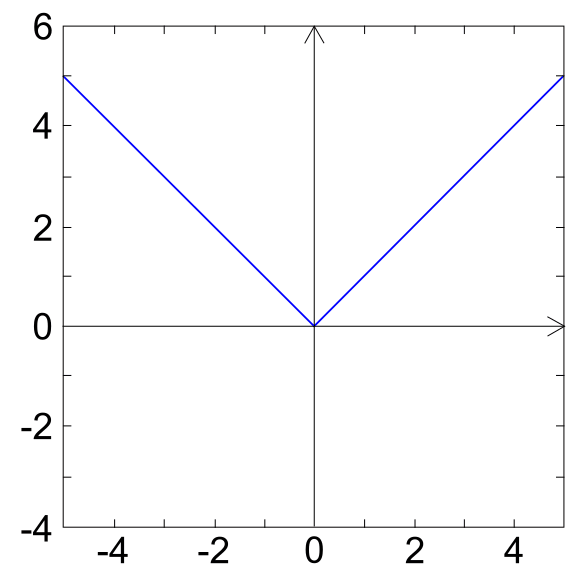
\includegraphics[width = 0.4\textwidth, height = 0.4\textwidth]{puntoangolos.png}
                \end{figure}
            \end{center}
        \subsubsection{Cuspide}
            $$\lim_{h \to 0^-} \textrm{R.I.} = \pm\infty \neq \mp\infty = \lim_{h \to 0^+} \textrm{R.I.}$$
            \begin{center}
                \begin{figure}[H]
                    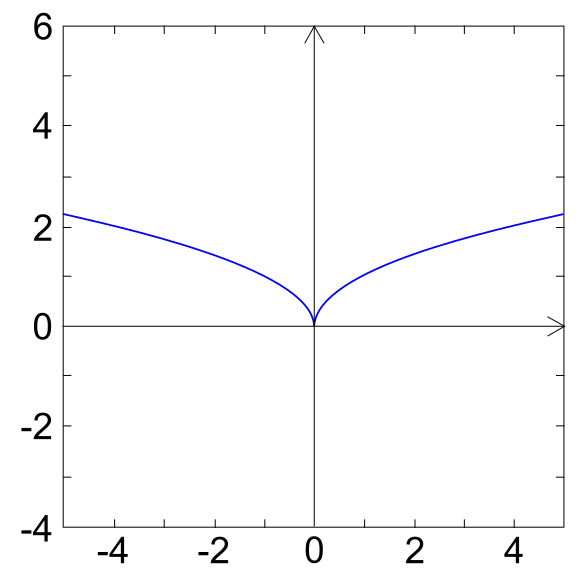
\includegraphics[width = 0.4\textwidth, height = 0.4\textwidth]{cuspide.png}
                \end{figure}
            \end{center}
        \subsubsubsection{Punto di flesso a tangente verticale}
            $$\lim_{h \to 0^-} \textrm{R.I.} = \pm\infty = \lim_{h \to 0^+} \textrm{R.I.}$$
            \begin{center}
                \begin{figure}[H]
                    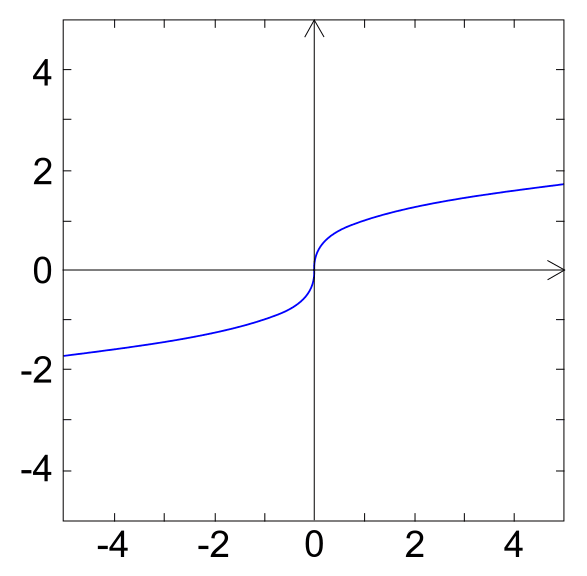
\includegraphics[width = 0.4\textwidth, height = 0.4\textwidth]{puntoflesso.png}
                \end{figure}
            \end{center}
    \subsection{Derivabilità e Continuità}
        $$\exists f^{'}\left(x\right) \Longrightarrow f \textrm{ continua }$$
    \subsection{Retta tangente in $x_0$}
        $$y = f\left(x_0\right) +f^{'}\left(x_0\right) \cdot \left(x - x_0\right)$$
    \subsection{Algebra delle derivate}
        Prese due funzioni $f, g$:
        \begin{itemize}
            \item $\left(f + g\right)^{'} = f^{'} + g^{'}$
            \item $\left(f \cdot g\right)^{'} = f^{'} \cdot g + f \cdot g^{'}$\\
                Nota come \textbf{regola di Leibnitz}
            \item $\left(\frac{f}{g}\right)^{'} = \frac{f^{'} \cdot g - f \cdot g^{'}}{g^2}$
        \end{itemize}
        \subsubsubsection{Dimostrazione regola di Leibnitz}
            $$\begin{array}{c}
                \D{x}\left(f\left(x\right) \cdot g\left(x\right)\right) = \lim_{h \to 0}\frac{f\left(x + h\right) \cdot g\left(x + h\right) - f\left(x\right) \cdot g\left(x\right)}{h} \\ \\ \\
                = \lim_{h \to 0}\frac{f\left(x + h\right) \cdot g\left(x + h\right) +\left[f\left(x + h\right) \cdot g\left(x\right) - f\left(x + h\right) \cdot g\left(x\right)\right]  - f\left(x\right) \cdot g\left(x\right)}{h} \\ \\ \\
                = \lim_{h \to 0}f\left(x + h\right) \cdot \frac{g\left(x + h\right) - g\left(x\right)}{h} + g\left(x\right) \cdot \frac{f\left(x + h\right) - f\left(x\right)}{h} \\ \\ \\
                = f\left(x\right) \cdot \D{x}g\left(x\right) + \D{x}{f\left(x\right)} \cdot g\left(x\right)
            \end{array}$$
        \subsubsection{Regola di Leibnitz ad n fattori}
            $$\D{x}\left(f \cdot f^1 \cdot ... \cdot f^n\right) = 
                \D{x}f \cdot f^1 ... \cdot f^n + f \cdot \D{x}f^1 \cdot ... \cdot f^n + ... + f \cdot f^1 \cdot ... \cdot \D{x}f^n
            $$
        \subsubsection{Regola di Leibnitz per la derivata n-esima}
            $$\D{x}{n}\left(f \cdot g\right) = \sum_{k = 0}^n \binom{n}{k}\D{x}{n-k}f \cdot \D{x}{k}g$$
    \subsection{Derivata della funzione composta}
        $$\D{x}\left(g \circ f\right)\left(x\right) =  \left(\D{x}g \circ f\right)\left(x\right) \cdot \D{x}f\left(x\right)$$
        \subsubsection{Dimostrazione}
            $$\begin{array}{c}
                \lim_{h \to 0}\frac{g\left(f\left(x + h\right)\right) - g\left(f\left(x\right)\right)}{h} \\ \\
                = \lim_{h \to 0}\frac{g\left(f\left(x + h\right)\right) - g\left(f\left(x\right)\right)}{h} \cdot \frac{f\left(x + h\right) - f\left(x\right)}{f\left(x + h\right) - f\left(x\right)} \\ \\
                = \lim_{h \to 0}\frac{g\left(f\left(x + h\right)\right) - g\left(f\left(x\right)\right)}{f\left(x + h\right) - f\left(x\right)} \cdot \frac{f\left(x + h\right) - f\left(x\right)}{h} \\ \\
                \Longrightarrow y = f\left(x\right), \, k = f\left(x + h\right) - f\left(x\right), \lim_{h \to 0}k = 0 \Longrightarrow \\ \\
                \lim_{k \to 0}\frac{g\left(y + k\right) - f\left(y\right)}{y + k - y} \cdot \lim_{h \to 0}\frac{f\left(x + h\right) - f\left(x\right)}{h} \\ \\
                = \D{y}g\left(y\right) \cdot \D{x}f\left(x\right) = \D{x}g\left(f\left(x\right)\right) \cdot \D{x}f \left(x\right)
            \end{array}$$
    \subsection{Derivata dell'inversa}
        $$g = f^{-1} \Longrightarrow \D{y}g = \frac{1}{\D{x}f\left(g\right)}$$
        \subsubsection{Dimostrazione}
            Il R.I. dell'inversa sarebbe $$\frac{\Delta x}{\Delta y} = \frac{1}{\frac{\Delta y}{\Delta x}}$$
            Quindi 
            $$\begin{matrix}
                \lim_{\Delta y \to 0}\textrm{R.I}_g = \lim_{\Delta x \to 0}\frac{1}{\textrm{R.I.}_f} \\ \\
                \D{y}g = \frac{1}{\D{x}f\left(f^{-1}\left(y\right)\right)}
            \end{matrix}$$
    \subsection{Punti stazionari}
        $$x \textrm{ punto stazionario} \Longleftrightarrow \D{x}f\left(x\right) = 0$$
        I punti stazionari possono essere \textbf{estremi locali} o \textbf{punti di flesso a tg. orizzontale}
    \subsection{Teorema di Fermat}
        $$f \textrm{derivabile}, f\left(x\right) \textrm{ estremo locale } \Longrightarrow \D{x}f\left(x\right) = 0$$
        \subsubsection{Dimostrazione}
            Analizziamo la dimostrazione con $f\left(x\right)$ massimo locale. La dimostrazione per il mimimo locale è analoga. \\
            $$\begin{matrix}
                \forall z \in \left(a, b\right), f\left(z\right) \leq f\left(x\right) \\ \\ 
                z < x \Longrightarrow \frac{f\left(z\right) - f\left(x\right)}{z - x} \geq 0 \Longrightarrow 
                    \D{x}f_{-}\left(x\right) = \lim_{z \to x^-}\frac{f\left(z\right) - f\left(x\right)}{z - x} \\ \\
                \Longrightarrow \D{x}f_{-}\left(x\right) \geq 0 \\ \\
                z > x \Longrightarrow \frac{f\left(z\right) - f\left(x\right)}{z - x} \leq 0 \Longrightarrow 
                    \D{x}f_{+}\left(x\right) = \lim_{z \to x^+}\frac{f\left(z\right) - f\left(x\right)}{z - x} \\ \\
                \Longrightarrow \D{x}f_{+}\left(x\right) \leq 0 \\ \\
                \Longrightarrow \D{x}f_{-}\left(x\right) = \D{x}f_{+}\left(x\right) = 0 = \D{x}f\left(x\right)
            \end{matrix}$$
    \subsection{Teorema del valore medio di Lagrange}
        $$\exists c \in \left(a, b\right) \textrm{ t.c. } \frac{f\left(b\right) - f\left(a\right)}{b - a} = \D{x}f\left(c\right)$$
        \subsubsection{Dimostrazione}
            Si può vedere come $\frac{f\left(b\right) - f\left(a\right)}{b - a}$ sia la pendenza della retta AB.
            L'equazione della retta è quindi
            $$y = f\left(a\right) + \frac{f\left(b\right) - f\left(a\right)}{b - a}\left(x-a\right)$$
            Consideriamo ora la funzione, continua e derivabile
            $$w\left(x\right) = f\left(x\right) - \left[f\left(a\right) + \frac{f\left(b\right) - f\left(a\right)}{b - a}\left(x-a\right)\right]$$
            Possiamo facilmente notare che $w\left(a\right) = w\left(b\right) = 0$. \\
            Per il teorema di Weiestrass $\exists x_1, x_2 \in \left[a, b\right]$ t.c. $M = f\left(x_1\right), m = f\left(x_2\right)$.
            Abbiamo ora diverse casistiche
            \begin{itemize}
                \item $M = m \Longrightarrow w\left(x\right) = k \forall x \in \left[a, b\right] \Longleftrightarrow \D{x}w\left(x\right) = 0 \forall x \in \left[a, b\right]$
                \item $M > m \Longrightarrow x_1 \neq a \neq b \textrm{ t.c. } \D{x}w\left(x_1\right) = 0 \textrm{ per il teorema di Fermat}$
            \end{itemize}
            Con 
            $$\D{x}w\left(x\right) = \D{x}f\left(x\right) - \frac{f\left(b\right) - f\left(a\right)}{b - a}$$
           Quindi
           $$\begin{array}{c}
            \exists c \in \left[a, b\right] \textrm{ t.c. } \D{x}w\left(x_0\right) = 0 \\ \\
            \Longrightarrow \D{x}f\left(c\right) - \frac{f\left(b\right) - f\left(a\right)}{b - a} = 0 \\ \\
            \Longrightarrow \D{x}f\left(c\right) = \frac{f\left(b\right) - f\left(a\right)}{b - a}
           \end{array}$$
    \subsection{Criterio di monotonia}
        $$\forall x \in \left(a, b\right) \D{x}f\left(x\right) \geq/\leq 0 \Longleftrightarrow f \textrm{ crescente/decrescente}$$
        \subsubsection{Dimostrazione}
            $$\begin{array}{c}
                \forall x, z \in \left(a, b\right), x < z \Longrightarrow \\ \\
                f \textrm{ crescente/decrescente} \Longleftrightarrow \frac{f\left(z\right) - f\left(x\right)}{z - x} \geq/\leq 0   \Longrightarrow \\ \\
                lim_{z \to x} \frac{f\left(z\right) - f\left(x\right)}{z - x} = \D{x}f\left(x\right) \geq/\leq 0
            \end{array}$$
            Abbiamo così mostrato l'implicazione da $f$ a $\D{x}f$. \\
            Dimostriamo ora anche l'implicazione opposta considerando il caso in cui $\D{x}f\left(x\right) \geq 0$.
            $$\begin{array}{c}
                \forall x, z \in \left(a, b\right) x < z \Longrightarrow \textrm{ per Lagrange } \exists c \in \left(x, z\right) 
                \textrm{ t.c. } \frac{f\left(z\right) - f\left(x\right)}{z - x} = \D{x}f\left(c\right) \geq 0 \textrm{ per ipotesi }  \\ \\
                \Longrightarrow z - x > 0 \Longrightarrow f\left(z\right) - f\left(x\right) \geq 0 \textrm{ Q.E.D}
            \end{array}$$
            Questo metodo ci permette di studiare anche la monotonia di alcune (non tutte!) successioni. 
    \subsection{Ricerca dei punti stazionari}
        Studiamo il comportamento di $\D{x}f\left(x_0 \in \left(a, b\right)\right) = 0$ in un intorno di $x_0$
        \begin{center}
            \begin{figure}[H]
                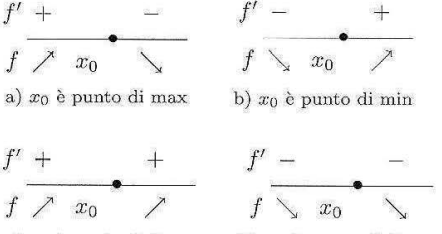
\includegraphics[width = 0.33\textwidth, height = 0.33\textwidth]{dermaxmin.png}
            \end{figure}
        \end{center}
        Ricordarsi di considerare anche $f\left(a\right)$ e $f\left(b\right)$
    \subsection{Teorema di de l'Hopital}
        $$f, g \textrm{ derivabili } \in \left(a, b\right) \wedge \forall x \in \left(a, b\right) \left(g\left(x\right) \neq 0 \wedge \D{x}g\left(x\right) \neq 0\right)$$
        $$\begin{array}{c}
            \lim_{x \to x_0^+} f\left(x\right) = \lim_{x \to x_0^-} g\left(x\right) = 0 \vee 
                \pm \infty \wedge \lim_{x \to x_0^+}\frac{\D{x}f\left(x\right)}{\D{x}g\left(x\right)} = l \in \mathbf{R} \\
                \Longrightarrow \lim_{x \to x_0^+} \frac{f\left(x\right)}{g\left(x\right)} = l
        \end{array}$$
    \subsection{Limite e derivata}
        $$\begin{array}{c}
            f: \left[a, b\right.\left.\right) \rightarrow \mathbf{R} \wedge f \textrm{ continua in } a 
                \wedge f \textrm{ derivabile } \in \left[a, b\right.\left.\right) \wedge \exists \lim_{x \to x_0^+} \D{x}f\left(x\right) = l \\
            \Longrightarrow \D{x}f_+\left(x_0\right) = l
        \end{array}$$
    \subsection{Derivata seconda}
        \subsubsection{Significato geometrico}
            Ci fornisce una misura del \textbf{grado di scostamento del grafico dall'andamento rettilinio}
            (ovvero quanto il grafico \textit{"curva"}). \\
            Ne consegue, $\forall x_0 \in X \textrm{ t.c. } \exists \D{x}{2}f\left(x_0\right)$ è relazionato 
            al cerchio con centro in $x_0$, nello specifico col raggio. \\
            $$\frac{1}{R\left(x\right)} = \frac{|\D{x}{2}f\left(x\right)|}{\left(1 + \D{x}f\left(x\right)^2\right)^{\frac{3}{2}}}$$
        \subsubsection{Convessità di una figura} 
            Data la figura $F$, questa è convessa se:
            $$\overline{P_1P_2} \in F \forall P_1, P_2 \in F \textrm{ t.c. } P_1 \neq P_2 \Longrightarrow F \textrm{ convessa }$$
        \subsubsection{Convessità di una funzione}
            \subsubsubsection{Definizione geometrica con l'epigrafico}
                Definiamo il concetto di epigrafico di una funzione come:
                $$\textrm{epi}_f = \{\left(x, y\right) \in \mathbf{R}^2 \mid x \in X, y \geq f\left(x\right)\}$$
                $$\textrm{epi}_f \textrm{ convesso } \in \left[a, b\right] \Longrightarrow f \textrm{ convessa } \in \left[a, b\right]$$
                In caso contrario è concava. \\
            \subsubsubsection{Definizione analitica}
                Definiamo prima l'equazione che definisce la \textbf{combinazione lineare convessa} di un segmento le cui x 
                sono comprese in $\left[a, b\right]$. 
                $$\begin{array}{l c r}
                     & t \in \left[0, 1\right] &  \\
                    z\left(t\right) = \left(1- t\right)a + tb & & f^*\left(t\right) = \left(1 - t\right)f\left(a\right) + tf\left(b\right)
                \end{array}$$
                Queste equazioni corrispondono alla corrispondenza fra il punto sulla curva e sul segmento fra gli estremi. \\
                $$f\left(z\left(t\right)\right) \leq f^*\left(t\right) \, \forall t \in \left[0, 1\right]\Longleftrightarrow f \textrm{ convessa } \in \left[a, b\right]$$
                Si parla di funzione \textbf{strettamente convessa} se ciò si verifica sempre anche per $<$
        \subsubsection{Continuità, derivabilità e convessità}
            $$f \textrm{ convessa o concava } \in \left[a, b\right] 
                \Longrightarrow f \textrm{ continua e derivabile da sinistra, destra } \in \left(a, b\right) \implies
            $$
            $$ \forall x \in \left(a, b\right), \exists \D{x}f\left(x\right) \textrm{ crescente } \in \left(a ,b\right) 
                    \Longleftrightarrow f \textrm{ convessa } \in \left(a, b\right) \Longleftrightarrow 
                    \exists \D{x}{2}f\left(x\right) \geq 0
            $$
            Ciò cambia in ovvi modi per la convessità e per le relazioni strette.
        \subsubsection{Convessità e tangente}
            $$\forall x_0 \in \left(a, b\right), \, \forall P \in \textrm{tangente}_{x_0}, 
                \, y_{P} \geq/\leq f\left(x\right) \forall x \in \left(a, b\right) \Longleftrightarrow f \textrm{ concava/convessa }$$
        \subsubsection{Punti di flesso}
            \subsubsubsection{Definizione}
                $$\begin{array}{c}\forall x_0 \in X, \exists \D{x}f\left(x\right) \vee \D{x}f\left(x\right) = \pm \infty \\ \\
                    \wedge \exists h > 0 \textrm{ t.c. } f \textrm{ concava/convessa } \in \left[x_0 - h, x_0\right] 
                    \wedge f \textrm{ convessa/concava } \in \left[x_0, x_0 + h\right] \\ \\
                    \Longleftrightarrow x_0 \textrm{punto di flesso}
                \end{array}$$
            \subsubsubsection{Punti di flesso e derivata seconda}
                $$\forall x \in X, \D{x}{2}f\left(x\right) = 0 \Longrightarrow x \textrm{ punto di flesso}$$ 
\newpage
\section{Derivate fondamentali}
    \begin{center}
        \begin{figure}[H]
            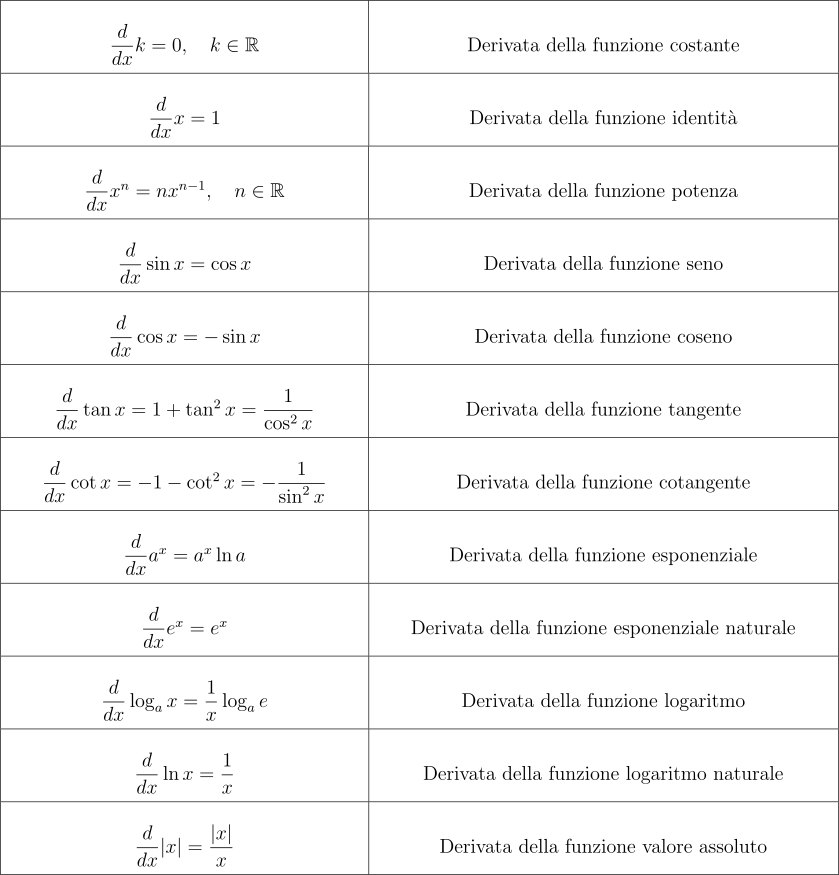
\includegraphics[width = \textwidth]{derivate.png}
        \end{figure}
    \end{center}
\newpage
\section{Studio di funzione}
    \begin{enumerate}
        \item Definire $D_f$
        \item Simmetrie e periodicità
        \item Intersezioni assi
        \item Intervalli di positività e negatività
        \item Valori agli estremi e asintoti
        \item Intervalli di monotonia, minimi e massimi (studio $\D{x}f\left(x\right)$)
        \item Intervalli di convessità e punti di flesso (studio $\D{x}{2}f\left(x\right)$)
        \item Grafico
    \end{enumerate}
\section{Calcolo differenziale e approssimazioni}
    \subsection{Linearizzazione e differenziale}
        La linearizzazione è un processo di approssimazione di come varia una funzione
        $f$ per una differenza $dx$. 
        $$\Delta f = f\left(x_0 + dx\right) - f\left(x_0\right) = \frac{f\left(x_0 + dx\right) - f\left(x_0\right)}{dx} \cdot dx \approx \D{x}f\left(x_0\right) \cdot dx \textrm{ per } dx \approx 0$$
        Ne consegue la definizione di \textbf{differenziale} di $f$ in $x_0$:
        $$df\left(x_0\right) = \D{x}f\left(x_0\right) \cdot dx$$
        Questa approssimazione presenta però un errore $\sigma\left(dx\right) \rightarrow 0$ per $dx \rightarrow 0$. \\
        Possiamo quindi scrivere:
        $$\lim_{dx \to 0}\frac{\Delta f}{dx} = \lim_{dx \to 0}\D{x}f\left(x_0\right) + \sigma\left(dx\right) 
            \Longrightarrow \lim_{dx \to 0}\Delta f - df\left(x_0\right) = \lim_{dx \to 0}dx \cdot \sigma\left(dx\right)$$
        L'algebra dei differenziali è equivalente all'algebra delle derivate
    \subsection{Infinitesimo}
        Prendiamo l'equazione di prima. Abbiamo che \\
        $$\lim_{dx \to 0}\frac{dx \cdot \sigma\left(dx\right)}{dx} = \lim_{dx \to 0}\sigma\left(dx\right) = 0$$
        Ovvero che $dx \cdot \sigma\left(dx\right)$ è un \textbf{infinitesimo di ordine superiore } rispetto a $dx$. \\
        Definiamo il concetto di infinitesimo
        $$\lim_{x \to x_0} \frac{f\left(x\right)}{g\left(x\right)} = 0 \Longleftrightarrow f\left(x\right) = o\left(g\left(x\right)\right)$$
        Nell'esempio di prima, abbiamo che $dx \cdot \sigma\left(dx\right) = o\left(dx\right)$ \\
        Possiamo quindi riscrivere l'equazione del paragrafo precedente come:
        $$\lim_{dx \to 0}\Delta f = \lim_{dx \to 0}df\left(x_0\right) + o\left(dx\right)$$
        Questa è detta \textbf{approssimazione} di $f$ al \textbf{prim'ordine}
        \subsubsection{Relazione con l'asintoto}
            Per $x \to 0$:
            $$f\left(x\right) \sim g\left(x\right) \Longleftrightarrow f\left(x\right) = g\left(x\right) + o\left(g\left(x\right)\right)$$
        \subsubsection{Algebra degli $o$-piccolo}
            \begin{itemize}
                \item $\lim_{x \to 0} o\left(x^n\right) \pm o\left(x^{n+1}\right) = o\left(x^n\right)$
                \item $\lim_{x \to \infty} o\left(x^n\right) \pm o\left(x^{n+1}\right) = o\left(x^{n+1}\right)$
                \item $k \cdot o\left(x\right) = o\left(k \cdot x\right) = o\left(x\right)$
                \item $f\left(x\right) \cdot o\left(g\left(x\right)\right) = o\left(f\left(x\right) \cdot g\left(x\right)\right)$
                \item $o\left(f\left(x\right)\right) \cdot o\left(g\left(x\right)\right) = o\left(f\left(x\right) \cdot g\left(x\right)\right)$
            \end{itemize}
    \subsection{Approssimazione polinomiale}
        L'idea di base è quella di approssimare il comportamento di una funzione 
        tramite un \textbf{polinomio di grado $n$}.
        Il processo col quale si \textit{"costruisce"} questo poliniomio, idealmente composto come $T_n\left(x\right) = c_0 + c_1x + ... x_nx^n$
        è un processo di matching 1 a 1. \\
        Praticamente cerchiamo valori delle costanti per i quali, dato $x_0$:
        $$\forall i \in \left[0, n\right], \, \D{x}{i}f\left(x_0\right) = \D{x}{i}T_n\left(x_0\right)$$
        Facile notare come, ad ogni derivata i-esima di $f$, a \textit{"controllare"} il valore 
        della derivata i-esima del polinomio sia un solo coefficiente, e
        come al crescere di $n$ migliori l'approssimazione, e come il limite 
        di $n$ è data da quante volte è derivabile $f\left(x_0\right)$. \\
        E' bene tenere a mente che esiste sempre un errore di approssimazione di ordine $o\left(x^n\right)$. \\
    \subsection{Polinomio di Taylor}
        Tutte le osservazioni del paragrafo prima ci portano alla conclusione che vogliamo 
        costruire il nostro poliniomio, l'unico per il quale valgono queste proprietà, detto polinomio di Taylor, secondo il seguente schema:
        $$f\left(x\right) = \left(T_n\left(x\right) = \sum_{i = 0}^{n}\frac{\D{x}{i}f\left(x_0\right)}{i!}\cdot\left(x-x_0\right)^i\right) + R_n\left(x\right)$$
        Dove $R_n$ rappresenta il resto dell'approssimazione. \\
        Notare come per arrivare al grado $n$ del polinomio occore che $f$ sia derivabile $n$-volte 
        in quel punto.
    \subsection{Calcolare il valore della derivata dal polinomio di Taylor}
            Data la funzione $f\left(x\right)$ il cui corrispondente polinomio di Taylor $T_{x_0,n}$ è 
            $$\sum_{i = 0}^n a_i \cdot \left(x - x_0\right)^i$$
            Possiamo calcolare il valore di $\D{x}{i}f\left(x_0\right) \, \forall i \leq n$ tramite la formula
            $$\D{x}{i}f\left(x_0\right) = a_i \cdot i!$$
        \subsubsection{Resto secondo Peano}
            Il resto secondo Peano ci fornisce l'entità del resto per $x \to x_0$,
            ed è utile usarlo quindi nei limiti.
            $$R_n\left(x_0\right) = o\left(\left(x-x_0\right)^n\right)$$
        \subsubsection{Resto secondo Lagrange}
            Nel caso in cui invece $x - x_0 = $ constante, risulta più utile usare il resto di Lagrange, 
            che si basa sul teorema di Lagrange, con la differenza che questa volta 
            $f$ deve essere derivabile $n+1$ volte. 
            $$\exists c \in \left(x_0, x\right) \textrm{ t.c. } R_n\left(x_0\right) 
                = \frac{\D{x}{n+1}f\left(c\right)}{\left(n+1\right)!} \cdot \left(x - x_0\right)^{n+1}$$
            Utile se $$\D{x}{n+1}f\left(x\right)$$ è limitata in $\left(x_0, x\right)$
    \subsection{Metodo di Newton}
        Il metodo di Newton è un metodo che ci permette di approssimare $x \in \left[a, b\right]$ tale che
        $f\left(x\right) = 0$. 
        $$\begin{array}{l} 
            \exists \D{x}f\left(x\right), \D{x}{2}f\left(x\right) \textrm{ con segno constante } \in \left[a, b\right] \\ \\
            f\left(a\right) \cdot f\left(b\right) < 0  \\ \\
            \D{x}{2}f\left(a\right) \cdot f\left(a\right) > 0 \Longrightarrow x_0 = a \\ \\
            \D{x}{2}f\left(b\right) \cdot f\left(b\right) > 0 \Longrightarrow x_0 = b \\ \\ 
            \implies \exists! c \in \left(a, b\right) \textrm{ t.c. } f\left(c\right) = 0 \wedge x_{n+1} = x_n - \frac{f\left(x_n\right)}{\D{x}f\left(x_n\right)} \to c \textrm{ per } n \to \infty
        \end{array}$$
        La successione converge a $c$ per difetto se $x_0 = a$, per eccesso se $x_0 = b$.
        \subsubsection{Dimostrazione}
            Essendo $f$ derivabile ne consegue che è anche continua. \\
            Per il teorema degli zeri, se si verifica la seconda ipotesi, allora 
            sappiamo che $\exists c \in \left(a, b\right) \textrm{ t.c. } f\left(c\right) = 0$. \\
            A garantirne l'unicità è la terza ipotesi, che implica la monotonia di $f \in \left[a, b\right]$. \\
            Per motivi di semplicità, supponiamo $f\left(a\right) < 0 \land f\left(a\right) \cdot \D{x}{2}f\left(a\right) \geq 0$. \\
            $$\begin{array}{l}
                f\left(a\right) \cdot f\left(b\right) < 0 \wedge f\left(a\right) < 0 \Longrightarrow f \textrm{ crescente } \in \left[a, b\right] \Longrightarrow \D{x}f\left(x\right) > 0 \land \D{x}{2}f\left(x\right) < 0 \\ \\
                g\left(x\right) = x - \frac{f\left(x\right)}{\D{x}f\left(x\right)} \Longrightarrow x_{n+1} = g\left(x_n\right) \Longrightarrow g\left(c\right) = c \\ \\
                \D{x}g\left(x\right) = 1 - \frac{\D{x}f\left(x\right)^2 - \D{x}{2}f\left(x\right) \cdot f\left(x\right)}{\D{x}f\left(x\right)^2} = \frac{\D{x}{2}f\left(x\right) \cdot f\left(x\right)}{\D{x}f\left(x\right)^2} \\ \\
                \Longrightarrow \forall x \in \left[a, b\right] \D{x}g\left(x\right) > 0 \Longrightarrow \forall x \in \left[a, c\right] g\left(x\right) \textrm{ monotona crescente }$$
            \end{array}$$
            Inoltre la successione è limitata superiormente in quanto 
            $$g\left(c\right) = c, x_n < c \implies g\left(x_n\right) < g\left(c\right) \implies g\left(x_n\right) < c \implies x_{n+1} < c \implies x_n \to \alpha$$
            Dimostriamo che converge a $c$.
            $$\begin{array}{c}
            \lim_{n \to \infty} x_n = \alpha \in \left[a, b\right] \Longrightarrow \lim_{n \to \infty} x_{n+1} = \lim_{n \to \infty} x_n - \frac{f\left(x_n\right)}{\D{x}f\left(x_n\right)} \\
                \Longrightarrow \textrm{ per la continuità di } f \, \, \, \alpha = \alpha - \frac{f\left(\alpha\right)}{\D{x}f\left(\alpha\right)} \Longrightarrow f\left(\alpha\right) = 0 \\
                \Longrightarrow f\left(\alpha\right) = 0 \wedge f\left(c\right) = 0 \Longrightarrow \textrm{ per l'unicità di } c \textrm{ ne consegue che } \alpha = c \Longrightarrow \lim_{n \to \infty} x_n = c
            \end{array}$$
\newpage
\section{Sviluppi noti di Taylor-MacLaurin}
    \begin{center}
        \begin{figure}[H]
            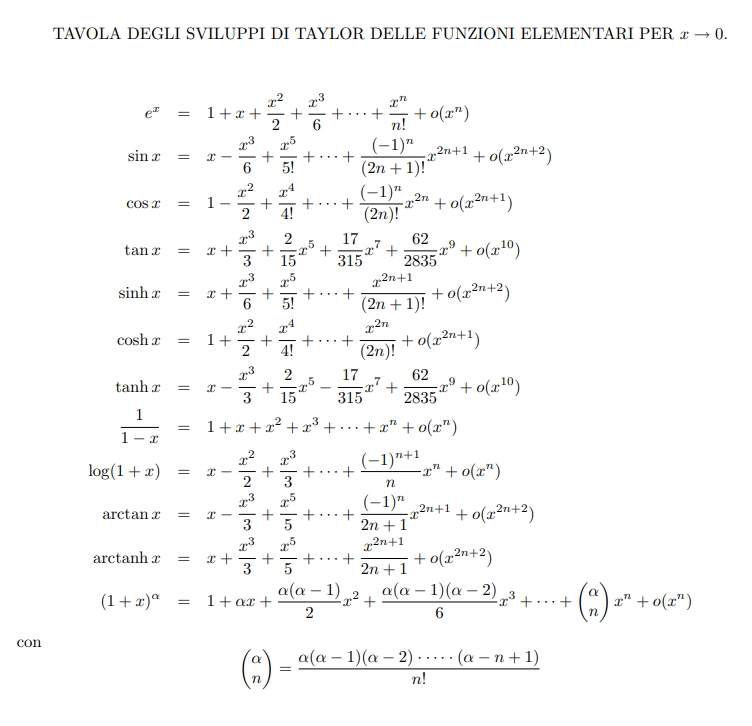
\includegraphics[width = \textwidth]{taylor.png}
        \end{figure}
    \end{center}
\newpage
\section{Funzioni iperboliche}
    \subsection{Iperbole}
        L'iperbole è la figura geometrica definita dalla funzione $x^2 - y^2 = 1$
        \begin{center}
            \begin{figure}[H]
                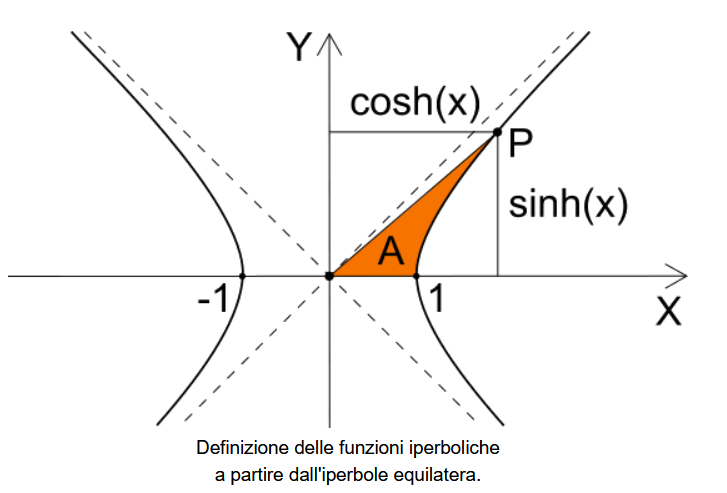
\includegraphics[width = 0.33\textwidth]{iperbole.png}
            \end{figure}
        \end{center}
    \subsection{Seno iperbolico}
        $$\begin{array}{c}
            \sinh: \mathbf{R} \rightarrow \mathbf{R} \\
            \sinh\left(x\right) = \frac{e^x-e^{-x}}{2} \\
            \D{x}\sinh\left(x\right) = \cosh\left(x\right)
        \end{array}$$
        \begin{center}
            \begin{figure}[H]
                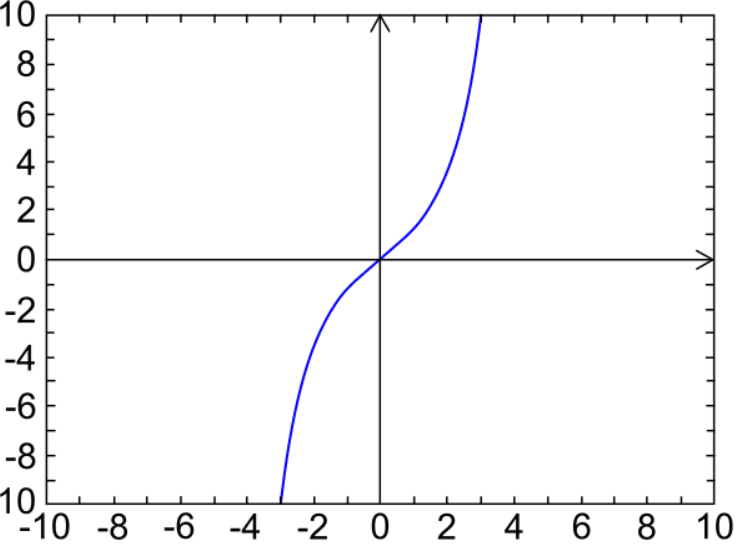
\includegraphics[width = 0.33\textwidth]{sinh.png}
            \end{figure}
        \end{center}
    \subsection{Coseno iperbolico}
        $$\begin{array}{c}
            \cosh: \mathbf{R} \rightarrow \left.\left[1, \infty\right.\right) \\
            \cosh\left(x\right) = \frac{e^x+e^{-x}}{2} \\
            \D{x}\cosh\left(x\right) = \sinh\left(x\right)
        \end{array}$$
        \begin{center}
            \begin{figure}[H]
                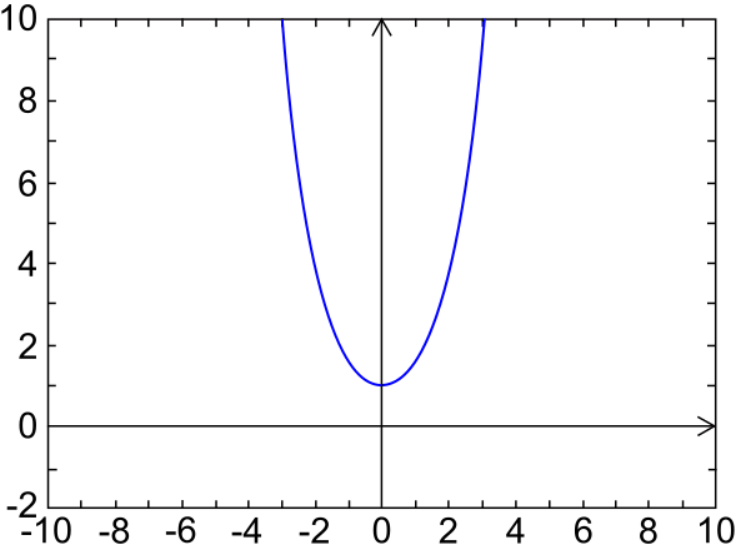
\includegraphics[width = 0.33\textwidth]{cosh.png}
            \end{figure}
        \end{center}
    \subsection{Tangente iperbolica}
        $$\begin{array}{c}
            \tanh: \mathbf{R} \rightarrow \left(-1, 1\right) \\
            \tanh\left(x\right) = \frac{\sinh\left(x\right)}{\cosh\left(x\right)} = \frac{e^2x - 1}{e^2x + 1} \\
            \D{x}\tanh\left(x\right) = 1 - \tanh^2\left(x\right) = \frac{1}{\cosh^2\left(x\right)}
        \end{array}$$
        \begin{center}
            \begin{figure}[H]
                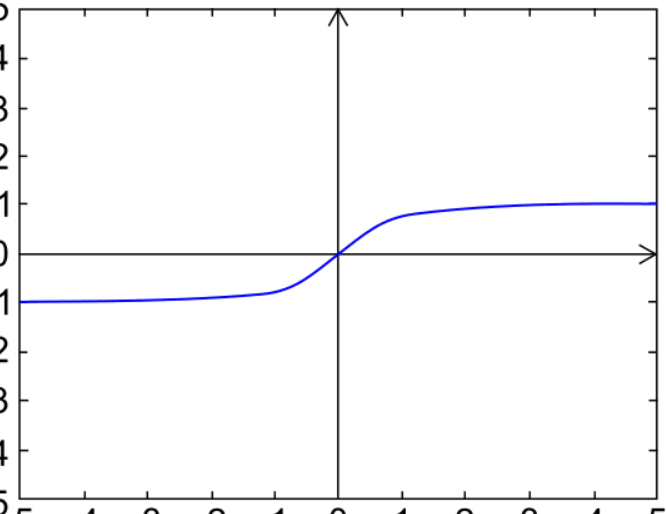
\includegraphics[width = 0.33\textwidth]{tanh.png}
            \end{figure}
        \end{center}
\newpage
\section{Numeri complessi}
    Il problema principale che vogliamo è avere un numero $z$ tale che $\sqrt{-1} = z$
    Definiremo i numeri che nascono da tale soluzione come \textbf{numeri complessi}, denotati nell'insieme $\mathbf{C} \supset \mathbf{R}$ \\
    \subsection{Numeri complessi come elementi di $\mathbf{R^2}$}
        Consideriamo l'elementi $\left(x, y\right) \in \mathbf{R^2}$, e definiamo le due operazioni base su di loro \\
        N.B.: Per questa definizione di $\mathbf{C}$, notiamo come i numeri complessi siano rappresentabili sul piano cartesiano.
        \subsubsection{Somma}
            $$+: \left(x_1, y_1\right) + \left(x_2, y_2\right) = \left(x_1 + x_2, y_1 + y_2\right)$$
            L'elemento neutro della somma è $\left(0, 0\right)$, l'inverso per $\left(x, y\right)$ è $\left(-x, -y\right)$
        \subsubsection{Prodotto}
            $$\cdot: \left(x_1, y_1\right) \cdot \left(x_2, y_2\right) = \left(x_1x_2 - y_1y_2, x_1y_2 + x_2y_1\right)$$ \\
            L'elemento neutro del prodotto è $\left(1, 0\right)$, l'inverso per $\left(x, y\right)$ è $\left(\frac{x}{x^2+y^2},\frac{-y}{x^2+y^2}\right)$
        \subsubsection{Quadrato di $\left(0, 1\right)$}
            $$\left(0, 1\right)^2 = \left(0, 1\right) \cdot \left(0, 1\right) = \left(-1, 0\right) = -1$$
    \subsection{Notazione con la $i$}
        Possiamo quindi definire $\left(0, 1\right) = i$, con $i^2 = -1$. \\
        Consideriamo ora il numero $\left(x, y\right) = \left(x, 0\right) + \left(0, 1\right) \cdot \left(y, 0\right)$. \\
        Possiamo quindi riscriverlo come $x + iy$.
        \subsubsection{Parte Immaginaria e parte Reale}
            Dato un numero $z = x + iy$:
            \begin{itemize}
                \item $x$ è detta \textbf{parte reale} di $z = \Re\left(z\right)$
                \item $y$ è detta \textbf{parte immaginaria} di $z = \Im\left(z\right)$
            \end{itemize}
    \subsection{Rappresentazione polare}
        Un numero complesso può essere visto anche come la coppia base/altezza di un triango
        di angolo $\Theta$ e raggio $\rho$
        \begin{figure}[H]
            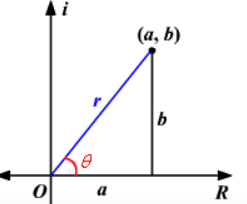
\includegraphics[width=.33\textwidth]{polar.png}
        \end{figure}
        Per proprietà trigonometriche, otteniamo che 
        \begin{itemize}
            \item $y = \rho \cdot \sin\Theta$
            \item $x = \rho \cdot \cos\Theta$
            \item $\tan\Theta = \frac{y}{x}$
        \end{itemize}
        Un numero $z = x + iy$ può essere riscritto come $\rho\left(\cos\Theta + i \cdot \sin\Theta\right)$
    \subsection{Identità di Eulero}
        $$z = x + iy = \rho\left(\cos\Theta + i \cdot \sin\Theta\right) = \rho e^{i \cdot \Theta}$$
        Ne conseugue l'identità fondamentale di eulero: 
        $$e^{i\pi} = -1 = i^2$$
    \subsection{Teorema fondamentale dell'Algebra}
        $$\forall P_n\left(z\right) = 0 \exists! z_1, ..., z_n \in \mathbf{C} 
            \textrm{ con le relative molteplicità }$$
    \subsection{Risolvere le equazioni di grado n in $\mathbf{C}$}
        Le radici di $z^n$ sono 
        $$\sqrt[n]{\rho}\cdot\left(\cos\left(\frac{2k\pi + \theta}{n}\right) + i\sin\left(\frac{2k\pi + \theta}{n}\right)\right)$$
        con $k \in \{0, ..., n-1\}$
    \subsection{Coniugato e modulo di $z$}
        \subsection{Coniugato}
            $$z = a + ib \implies \overline{z} = a - ib \implies z + \overline{z} = 2a, z - \overline{z} = 2bi$$
            $$\overline{z_1 + z_2} = \overline{z_1} + \overline{z_2}$$
            $$\overline{z_1 \cdot z_2} = \overline{z_1} \cdot \overline{z_2}$$
            $$\overline{z^{-1}} = \overline{z}^{-1}$$
        \subsection{Modulo}
            $$z = a + ib \implies |z| = \sqrt{a^2 + b^2}$$
            $$|z| = 0 \implies z = 0$$
            $$|z| = |\overline{z}|$$
            $$|\Re\left(z\right)|, \, |\Im\left(z\right)| \leq z$$
            $$\overline{z} \cdot z = |z|^2$$
\end{document}


